% Kozierok, ch. 21
\chapter{IP datagram encapsulation and formatting}
\label{chap:kozierok-ch21}


The primary job of the Internet Protocol (IP) is to deliver data between
devices over an internetwork. On its journey between two hosts in an
internetwork, this data may travel across many physical networks. To
help ensure that the data is sent and received properly, it is
\emph{encapsulated} within a message called an \emph{IP datagram}.
This datagram includes several fields that help manage the operation of
IP and ensure that data gets where it needs to go.

In this chapter, I take a look at how IP takes data passed to it from
higher layers and packages it for transmission. I begin with a general
discussion of IP datagrams and encapsulation. I then describe the
general format of IP datagrams, including the fields used in the IP
header and how they are interpreted.
I also include a brief discussion of IP datagram options and their use.


\begin{backgroundinfo}
This chapter assumes at least passing familiarity with IP addressing concepts, as outlined in
\cref{chap:kozierok-ch16,chap:kozierok-ch17,chap:kozierok-ch18,chap:kozierok-ch19,chap:kozierok-ch20}.
It also makes reference to the chapter on datagram fragmentation and reassembly (\cref{chap:kozierok-ch22}).
\end{backgroundinfo}


\begin{note}
IP datagrams are sometimes called IP packets.
Whether datagram or packet is the preferred term seems to depend on whom you ask; even the standards don't use one term exclusively.
On the other hand, I have seen IP datagrams called IP frames, and that's definitely not correct!
%\protect\hyperlink{ch01.html}{Chapter~1} describes these terms more completely}}.
\end{note}


%In \cref{sec:reference-models}, which described
In the introduction, where I described
OSI reference model concepts, I looked at several ways that protocols at various
layers in a networking protocol stack interact with each other.
One of the most important concepts in interprotocol operation is that of \emph{encapsulation}.
Most data originates within the higher layers of the OSI model.
The protocols at these layers pass the data down to lower layers for transmission, usually in the form of discrete messages.
Upon receipt, each lower-level protocol takes the entire contents of the message received and encapsulates it into its own message format, adding
a header and possibly a footer that contain important control information.

You might think of encapsulation as similar to sending a letter enclosed
in an envelope.
You write a letter and put it in an envelope with a name and address, but if you give it to a courier for overnight delivery;
the courier takes that envelope and puts it in a larger delivery envelope.
In a similar way, messages at higher networking layers are encapsulated in lower-layer messages, which can then in turn be further encapsulated.

Due to the prominence of TCP/IP, IP is one of the most important places
where data encapsulation occurs on a modern network. Data is passed to
IP typically from one of the two main transport layer protocols: the
Transmission Control Protocol (TCP) or User Datagram Protocol (UDP).
This data is already in the form of a TCP or UDP message with TCP or UDP
headers. This is then encapsulated into the body of an IP message,
usually called an \emph{IP datagram} or \emph{IP packet}.
Encapsulation and formatting of an IP datagram is also sometimes called \emph{packaging} -- again, the envelope is an obvious comparison.

\Cref{fig:ip-datagram-encapsulation} displays this entire process, which looks very similar to the drawing of
the OSI Reference Model as a whole, as shown in
\protect\hyperlink{ch05s03.htmlux5cux23osi_reference_model_data_encapsulation_e}{Figure~5-5} in \protect\hyperlink{ch05.html}{Chapter~5}.
As you can see, an upper-layer message is packaged into a TCP or UDP message.
This then becomes the payload of an IP datagram, shown here with only one header
(things can get a bit more complex than this). The IP datagram is then
passed down to layer~2, where it is encapsulated into some sort of local
area network (LAN), wide area network (WAN), or wireless LAN (WLAN)
frame, and then converted to bits and transmitted at the physical layer.

If the message to be transmitted is too large to pass through the
underlying network, it may first be fragmented. This is analogous to
splitting up a large delivery into multiple smaller envelopes or boxes.
In this case, each IP datagram carries only part of the higher-layer
message. The receiving device must reassemble the message from the IP
datagrams.


\begin{figure}
   \centering
   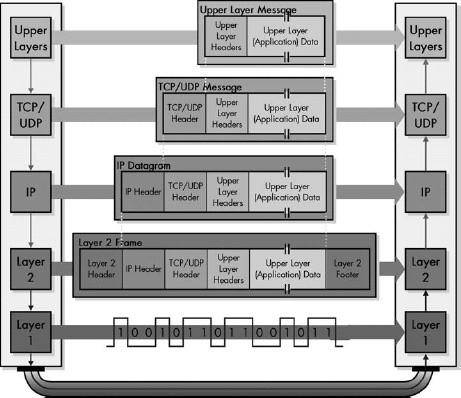
\includegraphics[width=.7\textwidth]{images/ip-datagram-encapsulation.jpg}
   \caption
      [IP datagram encapsulation]{
         IP datagram encapsulation -- The upper-layer message is packaged into a TCP or UDP message, which becomes the payload of an IP datagram.
         The IP datagram is then passed down to layer~2, where it is encapsulated in a LAN, WAN, or WLAN frame.
         It is then converted to bits and transmitted at the physical layer.
      }
   \label{fig:ip-datagram-encapsulation}
\end{figure}


The IP datagram is somewhat similar in concept to a frame used in
Ethernet or another data link layer, except that IP datagrams are
designed to facilitate transmission across an internetwork, while data
link layer frames are used only for direct delivery within a physical
network. The fields included in the IP header are used to manage
internetwork datagram delivery. This includes key information for
delivery, such as the address of the destination device, identification
of the type of frame, and control bits. The header follows a format that
you will examine shortly.

Once data is encapsulated into an IP datagram, it is passed down to the
data link layer for transmission across the current ``hop'' of the
internetwork. There it is further encapsulated, IP header and all, into
a data link layer frame such as an Ethernet frame. An IP datagram may be
encapsulated into many such data link layer frames as it is routed
across the internetwork; on each hop, the IP datagram is removed from
the data link layer frame and then repackaged into a new one for the
next hop. The IP datagram, however, is not changed (except for some
control fields) until it reaches its final destination.



Data transmitted over an internetwork using IP is carried in messages
called \emph{IP datagrams}. As is the case with all network protocol
messages, IP uses a specific
format for
its datagrams. Here, I will discuss the IP version 4 (IPv4) datagram
format,
which was defined in RFC 791 along with the rest of IPv4.

The IPv4 datagram is conceptually divided into two pieces: the
\emph{header} and the \emph{payload}. The header contains addressing
and control fields, while the payload carries the actual data to be sent
over the internetwork. Unlike some message formats, IP datagrams do not
have a footer following the payload.

Even though IP is a relatively simple, connectionless, and unreliable protocol, the IPv4 header carries a fair bit of information, which makes it rather large.
It is at least 20 bytes long, and with options it can be significantly longer.
The IP datagram format is described in next, as well as in \vref{tab:ipv4-flags,tab:ipv4-protocols}, and illustrated in \vref{fig:ipv4-datagram-format}.

\begin{description}
\item[Version (4 bits)]
   Identifies the version of IP used to generate the datagram.
   For IPv4, this is the number 4.
   This field ensures compatibility between devices that may be running different versions of IP.
   In general, a device running an older version of IP will reject datagrams created by newer implementations, under the assumption that the older version may not be able to interpret the newer datagram correctly.
\item[IP header length (4 bits)]
   Specifies the length of the IP header, in 32-bit words.
   This includes the length of any options fields and padding.
   The normal value of this field when no options are used is 5 (five 32-bit words or $5\times 4 = 20$ bytes).
   Contrast this with the longer Total Length field in this table.
\item[Type of service (1 byte)]
   A field designed to carry information to provide quality-of-service features, such as prioritized delivery for IP datagrams.
   This has not been as widely used as originally defined, and its meaning has been redefined for use by a technique called \emph{differentiated services} (DS), as discussed in \vref{sec:ip-datagram-tos}.
\item[Total length (2 bytes)]
   Specifies the total length of the IP datagram, in bytes.
   Since this field is 16 bits wide, the maximum length of an IP datagram is 65,535 bytes, though most are much smaller.
\item[Identification (2 bytes)]
   This field contains a 16-bit value that is common to each of the fragments belonging to a particular message;
   for datagrams originally sent unfragmented, it is still filled in so it can be used if the datagram must be fragmented by a router during delivery.
   The recipient uses this field to reassemble messages without accidentally mixing fragments from different messages.
   This is needed because fragments may arrive from multiple messages mixed together, since IP datagrams can be received out of order from any device.
   (See the discussion of IP message fragmentation in \cref{chap:kozierok-ch22}.)
\item[Flags (3 bits)]
   Three control flags, two of which are used to manage fragmentation (as described in the topic on fragmentation), and one that is reserved.
   See \vref{tab:ipv4-flags}.
\item[Fragment offset (13 bits)]
   When fragmentation of a message occurs, this field specifies the offset, or position, in the message where the data in this fragment goes in units of eight bytes (64 bits).
   The first fragment has an offset of 0.
   (See the discussion of fragmentation in \protect\hyperlink{ch27.html}{Chapter~27} for a description of how the field is used.)
\item[Time to live (1 byte)]
   This specifies how long the datagram is allowed to live on the network, in router hops.
   Each router decrements the value of the TTL field (reduces it by one) prior to transmitting it.
   If the TTL field drops to zero, the datagram is assumed to have taken too long a route and is discarded.
   (See \vref{sec:ip-datagram-ttl} for more information.)
\item[Protocol (1 byte)]
   Identifies the higher-layer protocol (generally either a transport layer protocol or encapsulated network layer protocol) carried in the datagram.
   \Vref{tab:ipv4-protocols} shows the protocol values of this field, which were originally defined by the IETF ``Assigned Numbers'' standard,
   RFC 1700, and are now maintained by the Internet Assigned Numbers Authority (IANA).
\item[Header checksum (2 bytes)]
   A checksum is computed over the header to provide basic protection against corruption in transmission.
   This is not the more complex cyclic redundancy check (CRC) code that's typically used by data link layer technologies such as Ethernet;
   it's just a 16-bit checksum.
   It is calculated by dividing the header bytes into words (a word is two bytes) and then adding them together.
   Only the header is checksummed; not the data.
   At each hop, the device receiving the datagram does the same checksum calculation, and if there is a mismatch, it discards the datagram as damaged.
\item[Source address (4 bytes)]
   This is the 32-bit IP address of the originator of the datagram.
   Note that even though intermediate devices such as routers may handle the datagram, they do not normally put their address into this field -- the address is always that of the device that originally sent the datagram.
\item[Destination address (4 bytes)]
   This is the 32-bit IP address of the intended recipient of the datagram.
   Again, even though devices such as routers may be the intermediate targets of the datagram, this field is always used to specify the ultimate destination.
\item[Options (variable)]
   One or more of several types of options may be included after the standard headers in certain IP datagrams, as discussed in \vref{sec:ip-datagram-options}.
\item[Padding (variable)]
   If one or more options are included, and the number of bits used for them is not a multiple of 32, enough 0~bits are added to pad out the header to a multiple of 32~bits (four bytes).
\item[Data (variable)]
   This is the data that will be transmitted in the datagram.
   It is either an entire higher-layer message or a fragment of one.
\end{description}


\begin{table}
   \centering
   \begin{tabular}{rrl}
      \textit{name}     & size (bits) & description \\[1ex]
      \textit{reserved} & 1           & not used\\
      \textit{DF}       & 1           & When set (1), the datagram should not be fragmented\\
      \textit{MF}       & 1           & When set (1), more fragments are to come in the fragmented message\\
   \end{tabular}
   \caption{IPv4 flags subfields}
   \label{tab:ipv4-flags}
\end{table}


\begin{table}
   \centering
   \begin{tabular}{rrl}
      value (hex) & value (dec) & protocol\\[1ex]
      00 & 0 & reserved\\
      01 & 1 & ICMP\\
      02 & 2 & IGMP\\
      %03 & 3 & GGP\\
      04 & 4 & IP-in-IP Encapsulation\\
      06 & 6 & TCP\\
      %08 & 8 & EGP\\
      11 & 17 & UDP\\
      2f & 47 & GRE\\
      32 & 50 & ESP extension header\\
      33 & 51 & AH extension header\\
      58 & 88 & EIGRP \\
      59 & 89 & OSPF \\
   \end{tabular}
   \caption{IPv4 protocol subfields}
   \label{tab:ipv4-protocols}
\end{table}


%\begin{note}
%The last two entries in \cref{tab:ipv4-protocols} are used when IPSec inserts additional headers into the datagram: the AH or ESP headers.
%%See \protect\hyperlink{ch29.html}{Chapter~29} for more information}}.
%\end{note}


\begin{figure}
   \centering
   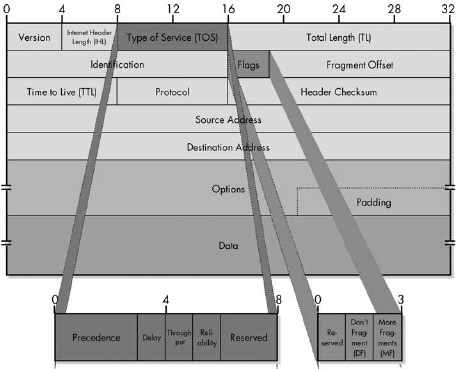
\includegraphics[width=.7\textwidth]{images/ipv4-datagram-format.jpg}
   \caption
      [IPv4 datagram format]
      {IPv4 datagram format -- This diagram shows the all-important IPv4 datagram format.
      The first 20 bytes are the fixed IP header, followed by an optional Options section, and a variable-length data area.
      Note that the Type of Service field is shown as originally defined in the IPv4 standard.}
   \label{fig:ipv4-datagram-format}
\end{figure}



\section{IP datagram time-to-live (TTL) field}
\label{sec:ip-datagram-ttl}

Let's look at the time-to-live (TTL) field.
Since IP datagrams are sent from router to router as they travel across an internetwork, a datagram could be passed from Router A to Router B to Router C, and then back to Router A.
This is called a \emph{routing loop}\index{routing loop}, and it's something that we don't want to happen.

To ensure that datagrams don't circle around endlessly, the TTL field was designed to contain a time value (in seconds),
which would be filled in when the datagram was originally sent.
Routers would decrease the time value periodically, and if it ever hit zero, destroy the datagram.
The TTL field was also designed to ensure that time-critical datagrams wouldn't become stale or pass their expiration date.

In practice, this field is not used in exactly this manner.
Routers today are fast and usually take far less than a second to forward a datagram, which makes it impractical to measure the time that a datagram lives.
Instead, this field is used as a \emph{maximum hop count} for the datagram.
Each time a router processes a datagram, it reduces the value of the TTL field by one.
If doing this results in the field being zero, the datagram is said to have expired, at which point it is dropped,
and usually an Internet Control Message Protocol (ICMP) Time Exceeded message is sent to inform the originator of the message that it has expired.
The TTL field is one of the primary mechanisms by which networks are protected from routing loops.
%(See the description of ICMP Time Exceeded messages in \protect\hyperlink{ch32.html}{Chapter~32} for more on how TTL helps IP handle routing loops.)





\section{IP datagram type of service (TOS) field}
\label{sec:ip-datagram-tos}

The Type-of-Service (TOS) field is a one-byte field that was originally intended to provide certain quality-of-service (QoS) features for IP datagram delivery.
It allowed IP datagrams to be tagged with information indicating not only their precedence, but also the preferred manner in which they should be delivered.
It was divided into a number of subfields, as shown in
\protect\hyperlink{ch21s02.htmlux5cux23original_definition_of_ipv_type_of_servi}{Table~21-4}
and
\protect\hyperlink{ch21s02.htmlux5cux23ipv4_datagram_format_this_diagram_shows_}{Figure~21-2}.

The lack of QoS features has been considered a weakness of IP for a long
time. But as you can see in
\protect\hyperlink{ch21s02.htmlux5cux23original_definition_of_ipv_type_of_servi}{Table~21-4},
these features were built into IP from the start. The fact is that even
though this field was defined in the standard in the early 1980s, it was
not widely used by hardware and software. For years, it was just passed
around with all zeros in the bits and mostly ignored.

The Internet Engineering Task Force (IETF), seeing the field unused,
attempted to revive its use. In 1998, RFC 2474 redefined the first six
bits of the TOS field to support a technique called
\emph{differentiated services} (DS). Under DS, the values in the TOS field are called
\emph{codepoints} and are associated with different service levels.
(See RFC 2474 for all the details.)


\begin{note}
Be sure to read the remainder of this chapter for more information on how IP options are used in datagrams and \cref{chap:kozierok-ch22} for some more
context on the use of fragmentation-related fields such as Identification, Fragment Offset, and More Fragments.
\end{note}


\begin{description}
   \item[Precedence (3 bits)]
      A field indicating the priority of the datagram.
      There were eight defined values, from lowest to highest priority:
      \begin{itemize}
         \item 000: routine
         \item 001: priority
         \item 010: immediate
         \item 011: flash
         \item 100: flash override
         \item 101: critical or ECP
         \item 110: internetwork control
         \item 111: network control
      \end{itemize}
   \item[D (1 bit)]
      Set to 0 to request normal delay in delivery; set to 1 if a low delay delivery is requested.
   \item[T (1 bit)]
      Set to 0 to request normal delivery throughput; set to 1 if higher throughput delivery is requested.
   \item[R (1 bit)]
      Set to 0 to request normal reliability in delivery; set to 1 if higher reliability delivery is requested.
   \item[Reserved (2 bits)]
      Not used.
\end{description}



\section{IP datagram options, and option format}
\label{sec:ip-datagram-options}


All IP datagrams must include the standard 20-byte header that contains key
information such as the source and destination address of the datagram,
fragmentation control parameters, length information, and more. In
addition to these invariable fields, the creators of IPv4 included the
ability to add \emph{options} that provide additional flexibility in
how IP handles datagrams. Use of these options is, of course, optional.
However, all devices that handle IP datagrams must be capable of
properly reading and handling them.

The IP datagram may contain zero, one, or more options, so the total
length of the Options field in the IP header is variable. Each of the
options can be a single byte or multiple bytes in length, depending on
how much information the option needs to convey. When more than one
option is included, they are concatenated and put into the Options field
as a whole. Since the IP header must be a multiple of 32 bits, a Padding
field is included if the number of bits in all options together is not a
multiple of 32 bits.

Each IP option has its own subfield format, generally structured as
shown in Tables
\protect\hyperlink{ch21s03.htmlux5cux23ipv_option_format}{Table~21-5}
and
\protect\hyperlink{ch21s03.htmlux5cux23ipv_options_option_type_subfields}{Table~21-6},
and illustrated in
\protect\hyperlink{ch21s03.htmlux5cux23ipv4_options_field_format_this_diagram_s}{Figure~21-3}.
For most options, all three subfields are used: Option
Type,
Option Length, and Option Data. For a few simple options, however, this
complex substructure is not needed. In those cases, the option type
itself communicates all the information required, so the Option Type
field appears, and the Option Length and Option Data subfields are
omitted.



Table~21-5.~IPv4 Option Format

\begin{longtable}[]{@{}lll@{}}
\toprule
Subfield Name & Size (Bytes) & Description\tabularnewline
\midrule
\endhead
Option Type & 1 & The Option Type subfield is divided into three
subsubfields, as shown in
\protect\hyperlink{ch21s03.htmlux5cux23ipv_options_option_type_subfields}{Table~21-6}.\tabularnewline
Option Length & 0 or 1 & For variable-length
options,
indicates the size of the entire option, including all three subfields
shown here, in bytes.\tabularnewline
Option Data & 0 or variable & For variable-length
options,
contains data to be sent as part of the option.\tabularnewline
\bottomrule
\end{longtable}



Table~21-6.~IPv4 Options: Option Type Subfields

\begin{longtable}[]{@{}lll@{}}
\toprule
Sub-Subfield Name & Size (Bytes) & Description\tabularnewline
\midrule
\endhead
Copied Flag & 1/8 (1 bit) & This bit is set to 1 if the option is
intended to be copied into all fragments when a datagram is fragmented;
it is cleared to 0 if the option should not be copied into
fragments.\tabularnewline
Option Class & 2/8 (2 bits) & Specifies one of four potential values
that indicate the general category into which the option belongs. In
fact, only two of the values are used: 0 is for Control options, and 2
for Debugging and Measurement.\tabularnewline
Option Number & 5/8 (5 bits) & Specifies the kind of option. 32
different values can be specified for each of the two option classes. Of
these, a few are more commonly employed. See
\protect\hyperlink{ch21s03.htmlux5cux23common_ipv_options}{Table~21-7}
for more information on the specific options.\tabularnewline
\bottomrule
\end{longtable}

\protect\hyperlink{ch21s03.htmlux5cux23common_ipv_options}{Table~21-7}
lists the most common IPv4 options, showing the option class, option
number, and length for each (a length of 1 indicates that an option
consists of only an Option Type field). The table also provides a brief
description of how each is used.




%\includegraphics{httpatomoreillycomsourcenostarchimages287855.png.jpg}

Figure~21-3.~IPv4 Options field format This diagram shows the full field
format for an IPv4 option. Note that a few simple options may consist of
only the Option Type subfield, with the Option Length and Option Data
subfields omitted.



Table~21-7.~Common IPv4 Options

\begin{longtable}[]{@{}lllll@{}}
\toprule
Option Class & Option Number & Length (Bytes) & Option Name &
Description\tabularnewline
\midrule
\endhead
0 & 0 & 1 & End of Options List & An option containing just a single
zero byte, used to mark the end of a list of options.\tabularnewline
0 & 1 & 1 & No Operation & A ``dummy option'' used as internal padding to
align certain options on a 32-bit boundary when required.\tabularnewline
0 & 2 & 11 & Security & An option provided for the military to indicate
the security classification of IP datagrams.\tabularnewline
0 & 3 & Variable & Loose Source Route & One of two options for source
routing of IP datagrams.\tabularnewline
0 & 7 & Variable & Record Route & Allows the route used by a datagram to
be recorded within the header for the datagram itself. If a source
device sends a datagram with this option in it, each router that handles
the datagram adds its IP address to this option. The recipient can then
extract the list of IP addresses to see the route taken by the datagram.
Note that the length of this option is set by the originating device. It
cannot be enlarged as the datagram is routed, and if it fills up before
it arrives at its destination, only a partial route will be
recorded.\tabularnewline
0 & 9 & Variable & Strict Source Route & One of two options for source
routing of IP datagrams.\tabularnewline
2 & 4 & Variable & Timestamp & Works similar to the Record Route option,
but each device puts in a timestamp, so the recipient can see how long
it took for the datagram to travel between routers. As with the Record
Route option, the length of this option is set by the originating device
and cannot be enlarged by intermediate devices.\tabularnewline
2 & 18 & 12 & Traceroute & Used in the enhanced implementation of the
traceroute utility, as described in RFC 1393. Also see
\protect\hyperlink{ch33.html}{Chapter~33}, which discusses ICMP
traceroute messages.\tabularnewline
\bottomrule
\end{longtable}


\begin{keyconcept}
Each IPv4 datagram has a 20-byte mandatory header and may also include one or more \emph{options}.
Each option has its own field format, and most are variable in size.
\end{keyconcept}

Normally, IP datagrams are routed without any specific instructions from devices about the path a datagram should take from the source to the destination.
It's the job of routers to use routing protocols and to figure out those details.
In some cases, however, it may be advantageous to have the source of a datagram specify the route a datagram takes through the network.
This process is called \emph{source routing}\index{source routing}.\footnote{Source routing is a huge security issue and must not be allowed on your network.}

There are two IP options that support source routing.
In each, the option includes a list of IP addresses that specify the routers that must be used to reach the destination.
When \emph{strict} source routing is used, the path specified in the option must be used exactly, in sequence,
with no other routers permitted to handle the datagram at all.
In contrast, \emph{loose} source routing specifies a list of IP addresses that must be followed in sequence,
but it allows intervening hops between the devices on the list.
(For full details on the exact structure used by each option type, please refer to RFC 791.)
